\documentclass[10pt,a4paper]{report}
\usepackage{graphicx}
\usepackage{color}
\usepackage{subcaption}
\usepackage[export]{adjustbox}
\usepackage{scrextend} 
\usepackage[inline]{enumitem}
\usepackage{xcolor}
\usepackage[utf8]{inputenc}
\usepackage{cite}
\usepackage[T2A]{fontenc}
\usepackage{csquotes}
\usepackage[backend=biber,style=numeric,sorting=none]{biblatex}

\title{Statistics problems}
\author{Iakovleva Alena, DSBA 202}
\date{2022}

\begin{document}
\maketitle

\begin{abstract}
In this paper I decided to collect a couple of problems from our statistics course in order to use this note in the future, as it is more convenient to read the tex document, rather then hand-written text.

\paragraph{What do I plan to include here?}
I will rewise a small amount of theory and then I will solve a couple of statistics problems. 
\end{abstract}

\tableofcontents 
\chapter{Theory}
\section{ANOVA}
Analysis of variance (ANOVA) is a popular tool that has an applicability and power that we can only start to appreciate in this course. The idea of analysis of variance is to investigate how variation in structured data can be split into pieces associated with components of that structure. We look only at one-way and two-way classifications, providing tests and confidence intervals which are widely used in practice.

\paragraph{One-way ANOVA}
One-way analysis of variance (one-way ANOVA) involves a continuous dependent variable and one categorical independent variable (sometimes called a factor, or treatment), where the k different levels of the categorical variable are the k different groups. We now introduce statistics associated with one-way ANOVA.

\paragraph{Two-way ANOVA}
Two-way analysis of variance (two-way ANOVA) involves a continuous dependent variable and two categorical independent variables (factors).

\subsection{Statistics associated with one-way ANOVA}

\paragraph{The ANOVA decomposition is}
\[ $\sum\limits_{j=1}^k  $\sum\limits_{i=1}^{n_j} (X_{ij} - \overline{X})^2  = $\sum\limits_{j=1}^k (\overline{X}_{.j} - \overline{X})^2 + 
$\sum\limits_{j=1}^k  $\sum\limits_{i=1}^{n_j} (X_{ij} - \overline{X}_{.j})^2 \] 
\\
\\
\\ $We have already discussed the jth sample mean and overall sample mean. The total variation is a measure of the overall (total) variability in the data from all k groups about the overall sample mean. The ANOVA decomposition decomposes this into two components.

\subsection{Some useful formulas}

\begin{enumerate}
\item Total variation
\[ $Total SS = B + W = $\sum\limits_{j=1}^k  $\sum\limits_{i=1}^{n_j} X_{ij}^2 - nX^2 \]

\item Residual (Error) SS
\[  $Residual (Error) SS = W =  $\sum\limits_{j=1}^k  $\sum\limits_{i=1}^{n_j} X_{ij}^2 - nX^2 - $\sum\limits_{j=1}^k n_j \overline{X}_{.j}^2  = $\sum\limits_{j=1}^k(n_j -1){S_j}^2 \]
\end{enumerate}

\subsection{One-way ANOVA table}
Typically, one-way ANOVA results are presented in a table as follows:
\\
\\
\begin{tabular}{ |r|c|c|c|c|c|}
\multicolumn{1}{r}{Source} &  \multicolumn{1}{c}{DF} & \multicolumn{1}{c}{SS} & \multicolumn{1}{c}{MS} & \multicolumn{1}{c}{F} & \multicolumn{1}{c}{p-value} \\
\cline{1-6} Factor & k - 1 & B & B/(k - 1) & $\frac{B/(k - 1)}{W/(n - k)} & p \\
\cline{1-6} Error & n - k & W & W/(n - k) & &  \\
\cline{1-6} Total & n - 1 & B + W & & &\\
\hline
\end{tabular} 

\section{Linear regression}

Regression analysis is one of the most frequently-used statistical techniques. It aims to model an explicit relationship between one dependent variable, often denoted as y, and one or several regressors (also called covariates, or independent variables), often denoted as x_1,...,x_p.
\\
\\
$The goal of regression analysis is to understand how y depends on x_1, . . . , x_p  $and to predict or control the unobserved y based on the observed x_1, . . . , x_p.  $We start with some simple examples with p = 1.

\begin{figure}[h]
\centering
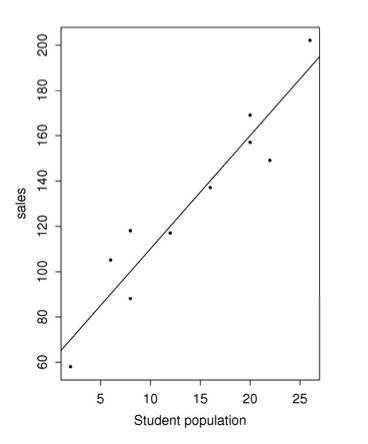
\includegraphics[width=0.5\textwidth]{/Users/aiakovleva/Documents/ACOS\ books/lab04/picture1.jpg}
\end{figure}

\subsection{Regression ANOVA}
We can\cite{tfidf1972} decompose the total variation of y in the simple linear regression model. It can be shown that the regression ANOVA decomposition is:

\[ $\sum\limits_{i=1}^n(y_i - \overline{y})^2 =  $\sum\limits_{i=1}^n \overline{\beta_i^2}(x_i - \overline{x}) + $\sum\limits_{i=1}^n 
(y_i - \overline{\beta_0} - \overline{\beta_1}x_i)^2 \]
\\
\\
$where, denoting sum of squares by ‘SS’ we have:
\\
\begin{enumerate} [label={\bullet}] 
\item Total SS is
\[  $\sum\limits_{i=1}^n (y_i - \overline{y})^2 =  $\sum\limits_{i=1}^n y_i^2 - n\overline{y}^2 \]

\item Regression (explained) SS is
\[  $\sum\limits_{i=1}^n \overline{\beta_i^2}(x_i - \overline{x})^2 =  \overline{\beta_i^2}($\sum\limits_{i=1}^n x_i^2 - n\overline{x}^2)\]

\item Residual (error) SS is
\[  $\sum\limits_{i=1}^n(y_i -  \overline{\beta}_0 - \overline{\beta}_1x_i)^2 = $Total SS - Regression SS\]

\end{enumerate}
\end{chapter}

\chapter{Practice}
\section{Problem 1}

\begin{figure}[h]
\centering

\includegraphics[width=0.7\textwidth]{/Users/aiakovleva/Documents/ACOS\ books/lab04/picture2.jpg}
\end{figure}

\flushleft
A dataset contains the annual cigarette consumption, x, and the corresponding mortality rate, y, due to coronary heart disease (CHD) of 21 countries. Some useful summary statistics calculated from the data are:
\\
\centering
\[  $\sum\limits_{i=1}^{21} x_i = 45110, \  $\sum\limits_{i=1}^{21} y_i = 042.2, \  $\sum\limits_{i=1}^{21} x_i^2 = 109957100, \\
$\sum\limits_{i=1}^{21} y_i^2 = 529321.58, \ $\sum\limits_{i=1}^{21} x_i y_i = 7319602.\]

\flushleft
Do these data support the suspicion that smoking contributes to CHD mortality? (Note the assertion ‘smoking is harmful for health’ is largely based on statistical, rather than laboratory, evidence.)
\\
\[ $\overline{\beta}_1 = {\frac{\sum\limits_i(x_i - \overline{x})(y_i - \overline{y})}{ \sum\limits_i(x_i - \overline{x})^2}} = \frac{7319602 - 45110 * 3042.2/21}{109957100 - (45110)^2/21} = 0.06 \]
\\
\[ $\overline{\beta}_0 = 15.77\]
\\
Since t = 0.06/0.01475 = 4.068 > 2.54 = t_{0.01}, $19, we reject the hypothesis β1 = 0 at the 1 \% significance level and we conclude that there is strong evidence that smoking contributes to CHD mortality.

\end{section}
\section{Problem 2, Histogram}
\begin{figure}[h]
\centering
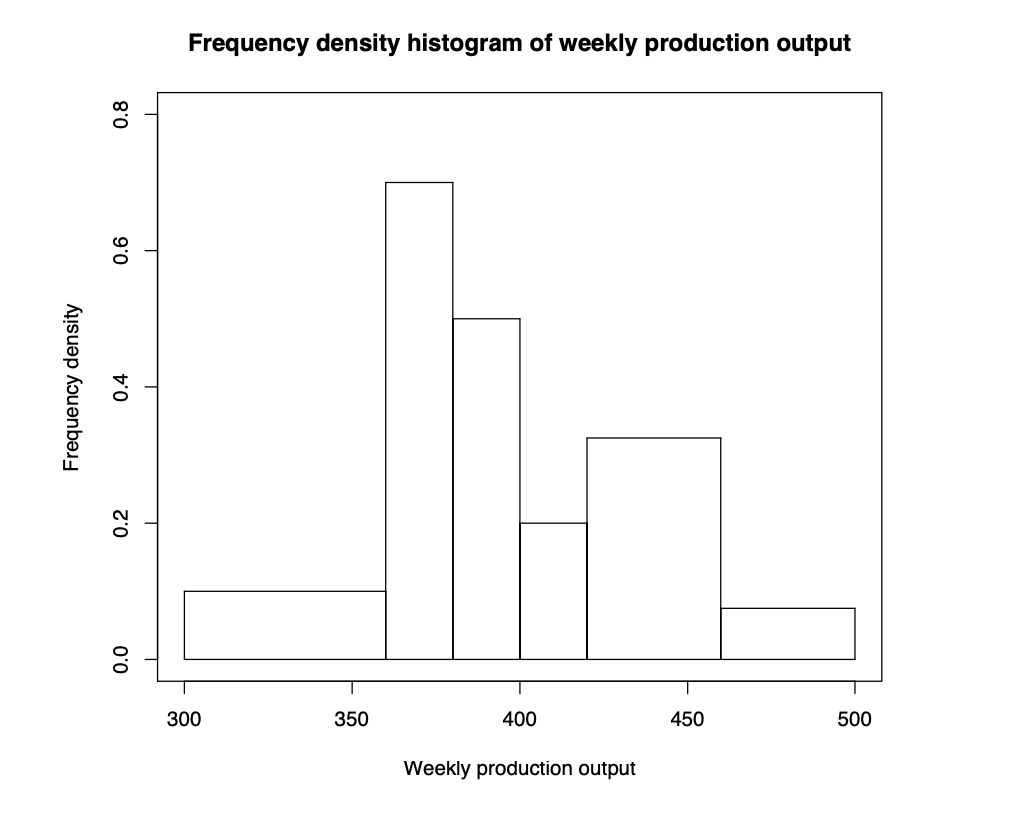
\includegraphics[width=0.9\textwidth]{/Users/aiakovleva/Documents/ACOS\ books/lab04/picture3.jpg}
\end{figure}

\begin{tabular}{ |r|c|c|c|c|c|}
\multicolumn{1}{r}{Class interval} &  \multicolumn{1}{c}{Interval width} & \multicolumn{1}{c}{Frequency} & \multicolumn{1}{c}{Frequency density} & \multicolumn{1}{c}{Cumulative frequency} \\
\cline{1-6} [300, 360) & 60 & 6 & 0.100 & 6  \\
\cline{1-6} [360, 380) & 20 & 14 & 0.700 & 20  \\
\cline{1-6} [380, 400) & 20 & 10 & 0.500 & 30  \\
\cline{1-6} [400, 420) & 20 & 4 & 0.200 & 34  \\
\cline{1-6} [420, 460) & 40 & 13 & 0.325 & 47  \\
\cline{1-6} [460, 500) & 40 & 3 & 0.075 & 50  \\
\hline
\end{tabular} 

\paragraph{}The table above includes two additional columns: (i.) ‘Frequency density’ – obtained by calculating ‘frequency divided by interval width’ (for example, 6/60 = 0.100), and (ii.) ‘Cumulative frequency’ – obtained by simply determining the running total of the class frequencies (for example, 6 + 14 = 20). Note the final column is not required for a histogram per se, although the computation of cumulative frequencies may be useful when determining medians and quartiles (to be discussed later in this chapter). \cite{Sulsky1994}\\
\\
\\
\paragraph{}To construct the histogram, adjacent bars are drawn over the respective class intervals such that the area of each bar is proportional to the interval frequency. This explains why equal bin widths are desirable since this reduces the problem to making the heights proportional to the interval frequency. However, you may be told to use a particular number of bins or bin widths, such that the bins will not all be of equal width. In such cases, you will need to compute the frequency density as outlined above. \footnote{Wow, this is my comment}
\\

\chapter{Thanks}

My quote: 
''Thanks for the opportunity to show how I can use Latex'' \linebreak[4]

\textit{}

\Huge 
So, that is it! I am done with my document! I hope that you liked it!
\normalsize

\begin{figure}[h]
\centering

\includegraphics[width=0.5\textwidth]{/Users/aiakovleva/Documents/ACOS\ books/lab04/picture4.jpg}
\end{figure}

\clearpage

\begin{thebibliography}{3}
\bibitem{Sulsky1994}
Sulsky D., Chen Z., Schreyer H. L.  A particle method for history-dependent materials // Computer Methods in Applied Mechanics and Engineering. --- 1994, V. 118. --- P. 179--196.
\bibitem{Vshivkov}
Григорьев Ю. В., Вшивков В. А., Федорук, М. П. Численное моделирование методами частиц в ячейках. --- Новосибирск : Издательство СО РАН. --- 2004. --- 360 c.
\bibitem{LiuLiu}
Liu G. R., Liu M. B. Smoothed particle hydrodynamics: a meshfree particle method. --- Singapore : World Scientific Publishing. --- 2003. --- 449 p.
\end{thebibliography}

\end{document}